\documentclass[a4paper]{jarticle}
\usepackage{comment}
\usepackage[top=30truemm,bottom=30truemm,left=30truemm,right=30truemm]{geometry}
\usepackage{here}
\usepackage[dvipdfmx]{graphicx}
\usepackage[utf8]{inputenc}
\usepackage{listings,jlisting}
\lstset{tabsize=4}
\begin{document}
\section{課題1}
\begin{comment}
次のC言語のプログラムを字句解析すると、どのように分解され、それぞれは「名前」、「予約語」、「定数」、「記号」のどれに分類されるか?分解した結果と分類を示せ。定数についてはその値も示せ。同じ字句については、初出のところだけで説明すればよい。
\begin{lstlisting}
int main(int argc, char *argv[]){
	int ch;
	while((ch = getchar()) != -1){
		if((ch >= 'a') && (ch <= 'z'))ch = ch - 0x20;
		putchar(ch);
	}
}
\end{lstlisting}
\end{comment}
\begin{lstlisting}
int		予約語
main	名前
(		記号
int
argc	名前
,		記号
char	予約語
*		記号
argv	名前
[		記号
]		記号
)		記号
{		記号
int
ch		名前
;		記号
while	予約語	
(
(
ch
=		記号
getchar	名前
(
)
)
!=		記号
-1		定数(-1)
)
{
if		予約語
(
(
ch
>=		記号
'a'		定数(97)
)
&&		記号
(
ch
<=		記号
'z'		定数(122)
)
)
ch
=
ch
-		記号
0x20	定数(32)
;
putchar	名前
(
ch
)
;
}
}
\end{lstlisting}
\section{課題2}
\begin{comment}
教科書39ページの演習問題3.1$\sim$3.3を解け。問題3.1では、複数の非終端記号が1つの正規表現にまとめられる理由も示すこと。問題3.2では、このオートマトンを得た根拠も示すこと。問題3.3では、最終結果だけでなく、途中の過程も詳細に示すこと。
\setcounter{subsection}{2}
\end{comment}
\section*{演習問題}
\setcounter{section}{3}
\subsection{次のBNFで表される定数を正規表現で表しなさい。}
\begin{lstlisting}
浮動小数点数	→	符号部	数字列1	.	数字列0	E	符号部	数字列1
符号部			→	-|+|ε
数字列1			→	数字|数字列1	数字
数字列0			→	数字列1|ε
\end{lstlisting}
\begin{eqnarray*}
\bigl[ - | + | \epsilon \bigr] 数字 \{ 数字 \} . \{ 数字 \} E \bigl[ - | + | \epsilon \bigr] 数字 \{ 数字 \} \nonumber
\end{eqnarray*}
正規表現では、BNFの複数の非終端記号を連接によってひとつにまとめて表現することができる。
\subsection{演習3.1の正規表現を非決定性有限オートマトンで表しなさい。}
まず、開始状態Sを作る。
\begin{comment}
\begin{figure}[H]
 \begin{center}
  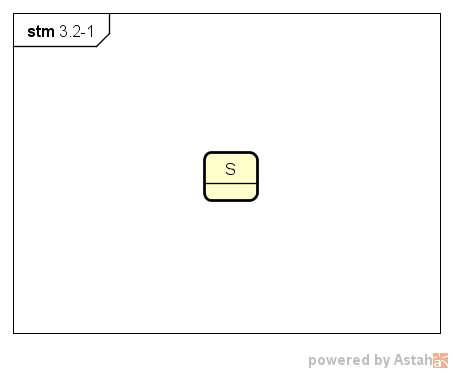
\includegraphics{Automatonfig/3-2-1.png}
 \end{center}
\end{figure}
\end{comment}
\subsection{演習3.2の非決定性有限オートマトンを決定性有限オートマトンに変換しなさい。}
\end{document}
